% !TeX program = xelatex
% 以 TikZ 绘制的原创装饰封面，不复制教材封面图。
\documentclass[tikz,border=0pt]{standalone}
\begin{document}
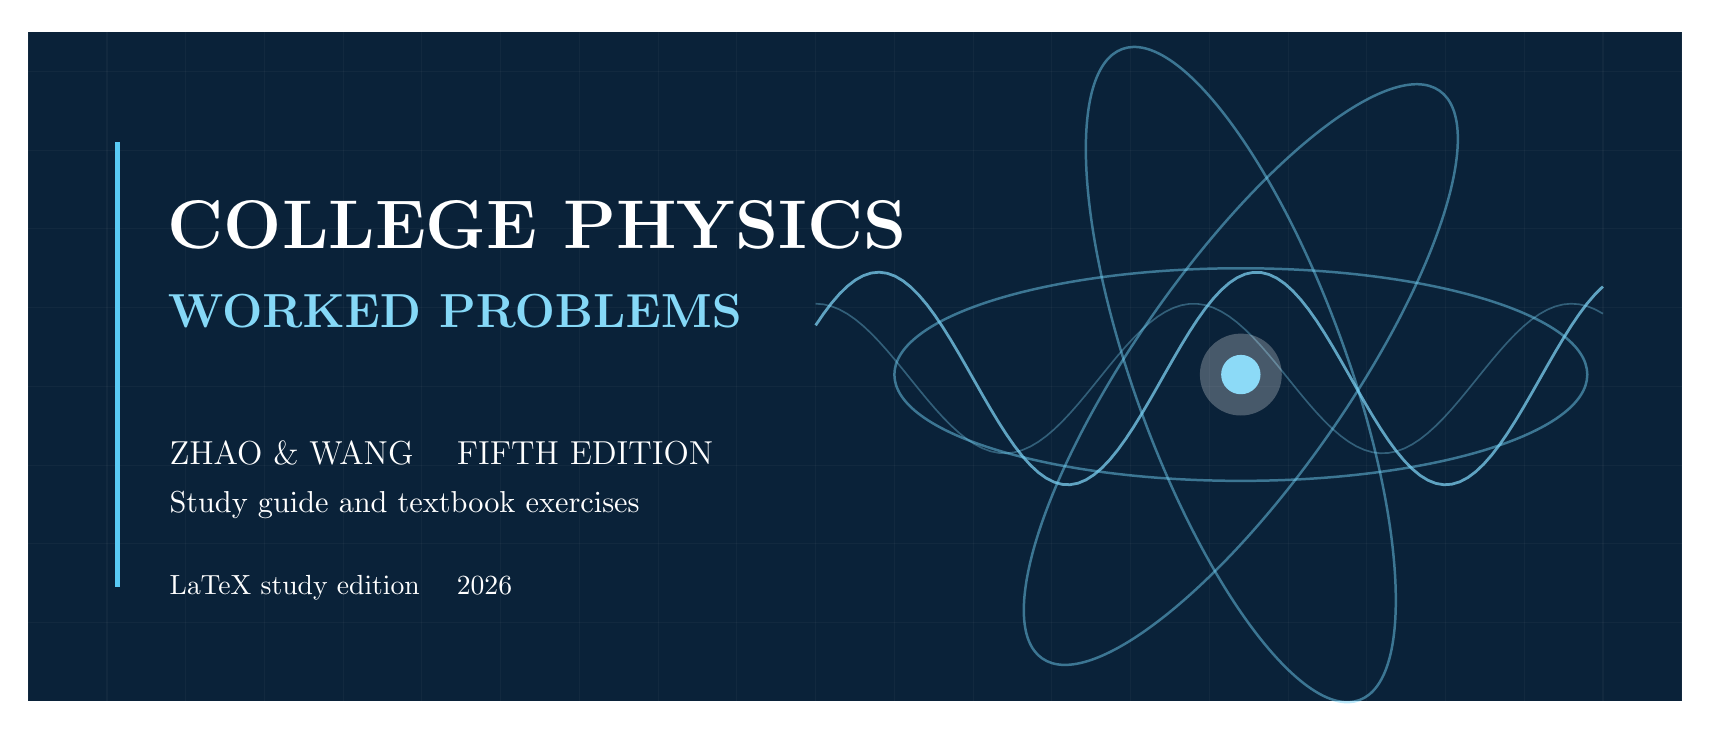
\begin{tikzpicture}[x=1cm,y=1cm]
  \path[fill={rgb,255:red,10;green,34;blue,57}] (0,0) rectangle (21,8.5);
  \foreach \i in {0,1,...,21} {\draw[white,opacity=.035] (\i,0)--(\i,8.5);}
  \foreach \j in {0,1,...,8} {\draw[white,opacity=.035] (0,\j)--(21,\j);}
  \draw[cyan!50!white,opacity=.72,line width=1pt]
    plot[domain=10:20,samples=100] (\x,{4.1+1.35*sin(75*\x)});
  \draw[cyan!50!white,opacity=.34,line width=.6pt]
    plot[domain=10:20,samples=100] (\x,{4.1+.95*sin(75*\x+60)});
  \begin{scope}[shift={(15.4,4.15)}]
    \foreach \angle in {0,55,110}{
      \draw[rotate=\angle,cyan!55!white,opacity=.48,line width=.9pt]
        (0,0) ellipse[x radius=4.4,y radius=1.35];
    }
    \fill[cyan!60!white] (0,0) circle (.25);
    \fill[white,opacity=.25] (0,0) circle (.52);
  \end{scope}
  \fill[cyan!65!white] (1.1,1.45) rectangle (1.17,7.1);
  \node[anchor=west,text=white,font=\bfseries\fontsize{33}{39}\selectfont]
    at (1.65,6.05) {COLLEGE PHYSICS};
  \node[anchor=west,text=cyan!48!white,font=\bfseries\fontsize{19}{25}\selectfont]
    at (1.65,4.95) {WORKED PROBLEMS};
  \node[anchor=west,text=white!75,font=\fontsize{13}{18}\selectfont]
    at (1.67,3.15) {ZHAO \& WANG \quad FIFTH EDITION};
  \node[anchor=west,text=white!65,font=\fontsize{11}{15}\selectfont]
    at (1.67,2.5) {Study guide and textbook exercises};
  \node[anchor=west,text=white!60,font=\fontsize{10}{13}\selectfont]
    at (1.67,1.45) {LaTeX study edition \quad 2026};
\end{tikzpicture}
\end{document}
